\documentclass[a4paper]{article}
\usepackage[czech]{babel}
\usepackage{graphicx}
\usepackage{tabularx}
\usepackage{hyperref}
\usepackage[utf8]{inputenc}
\usepackage[T1]{fontenc}
\pagenumbering{gobble}

\makeatletter
\g@addto@macro{\UrlBreaks}{\UrlOrds}
\makeatother


\begin{document}
\title{Stav půdy v ČR}
\author{Jiří Kalvoda}
\maketitle

Stav půdy je již poměrně delší dobu dobře monitorovaný a zkoumaný.
Její kvalit ovlivňuje způsob zemědělství na daném místě v minulosti a klimatické změny a metrologické jevy.
Dobrý stav je nutnou podmínkou k funkčnímu konkurenceschopnému zemědělství a v globálním měřítku tedy i k možnosti adekvátní výživy celé populace.
Proto je nutné o půdu usilovně a v dlouhodobém měřítku pečovat.

V ČR je $53.6\%$ rozlohy považováno za zemědělskou půdu.
Z nichž je zhruba $70\%$ zorněno.
Ovšem v poslední době je nemalé  množství půdy (a to i v oblastech, kde je velikce kvalitni) nevratně poničeno zástavbou (mezi lety 1966 a 2007 se jedná o $6\%$.
Zábor půdy má pak vliv na retenční kapacitu krajiny, tedy schopnost krajiny zadržovat vodu.

Způsob užívání zemědělské techniky má vliv na  utužování půdy. Jedná se o snižování objemu půdy (na daném prostoru) a tedy snížení pórovitosti půdy.
Statisticky v čR je tento trend skutečně prokázán.
Dalši hrozbou ke které má aktuální stav sklony je omezení vázání živin do půdy, tedy půdní sorpce. Ta v dlouhodobém hledisku zhoršuje podmínky pro pěstování a tedy snižuje úrodnost.
Další probíhající změnou je snižování pH půdy, vlivem intenzifikace zemědělství.

Důležitou složkou půdy je organická hmota v ní obsažená.
Její množství je sice stabilní, ovšem de průzkumů se snižuje její kvalita.
Pro její udržení je třeba správně obohacovat půdu o snadno rozložitelné složky (rostlinné zbytky, hnůj, kompost).

V poslední době také dochází k snižování zásob podzemní vody (vlivem dlouhodobého sníženého úhrnu srážek a zhoršení zadržovacích schopností půdy), které máá mimo jiné vliv na zvýšení množství  eroze.

\begin{figure}[tb]
\centering
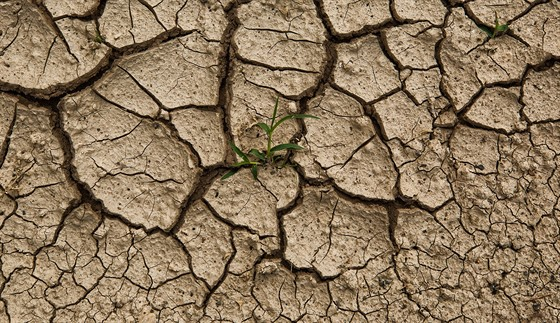
\includegraphics[width=0.5\textwidth]{puda.jpg}
	\caption{Půda v kritickém stavu sucha}
\end{figure}

Vzhledem k předchozím odstavcům lze tedy prohlásit, že výzkumy se shodují na tom, že dochází k výraznému zhoršení kvality půd, zejména zasazovaci schopnosti.
Degradační procesy se totiž obvykle vzájemně doplňují a podporují.
Například omezení infiltrace vody zrychlí odtok vody po povrchu, který umožní vodní erozi, jejímž důsledkem je ztráta organické hmoty a zhoršení půdní struktury.
Proto je nutné se systematicky věnovat zamezením těchto rušivých elementu a půdní fond podporovat.
například je vhodné střídat plodiny pěstované na dané části pudy (a tím i postupy obdělávání), zabraňovat erozi správným obděláváním a nevykořisťovat pudu masivním a neuváženým zemědělstvím.

\section*{Zdroje}


\begin{itemize}
	\item 
\url{https://www.mzp.cz/cz/articles_091123_Zemedelec}
\item
\url{http://eagri.cz/public/web/mze/puda/novinky/trendy-pud-v-cr-vysledky-vyzkumu.html}
\item
\url{https://www.idnes.cz/ekonomika/domaci/sucho-agrarni-analytik-komentar-esej-klimaticka-zmena-zemedelstvi.A190914_141532_ekonomika_rts}
\item
\url{https://www.uroda.cz/aktualni-stav-pud-v-ceske-republice/}
\item\url{https://www.cuzk.cz/O-resortu/Nemoforum/Akce-Nemofora/Seminare/BPEJ-a-pozemkove-upravy/01122016_BPEJ_Vopravil_Khel.aspx}
\end{itemize}
\end{document}
